%%%%%%%%%%%%%%%%%%%%%%%%%%%%%%%%%%%%%%%%%%%%%%%%%%%%%%%%%%%%%%%%%%%%%
% SLIDE 0: OVERVIEW SLIDE
%%%%%%%%%%%%%%%%%%%%%%%%%%%%%%%%%%%%%%%%%%%%%%%%%%%%%%%%%%%%%%%%%%%%%
\begin{frame}[fragile]\frametitle{Program at a Glance}
		\begin{center}
		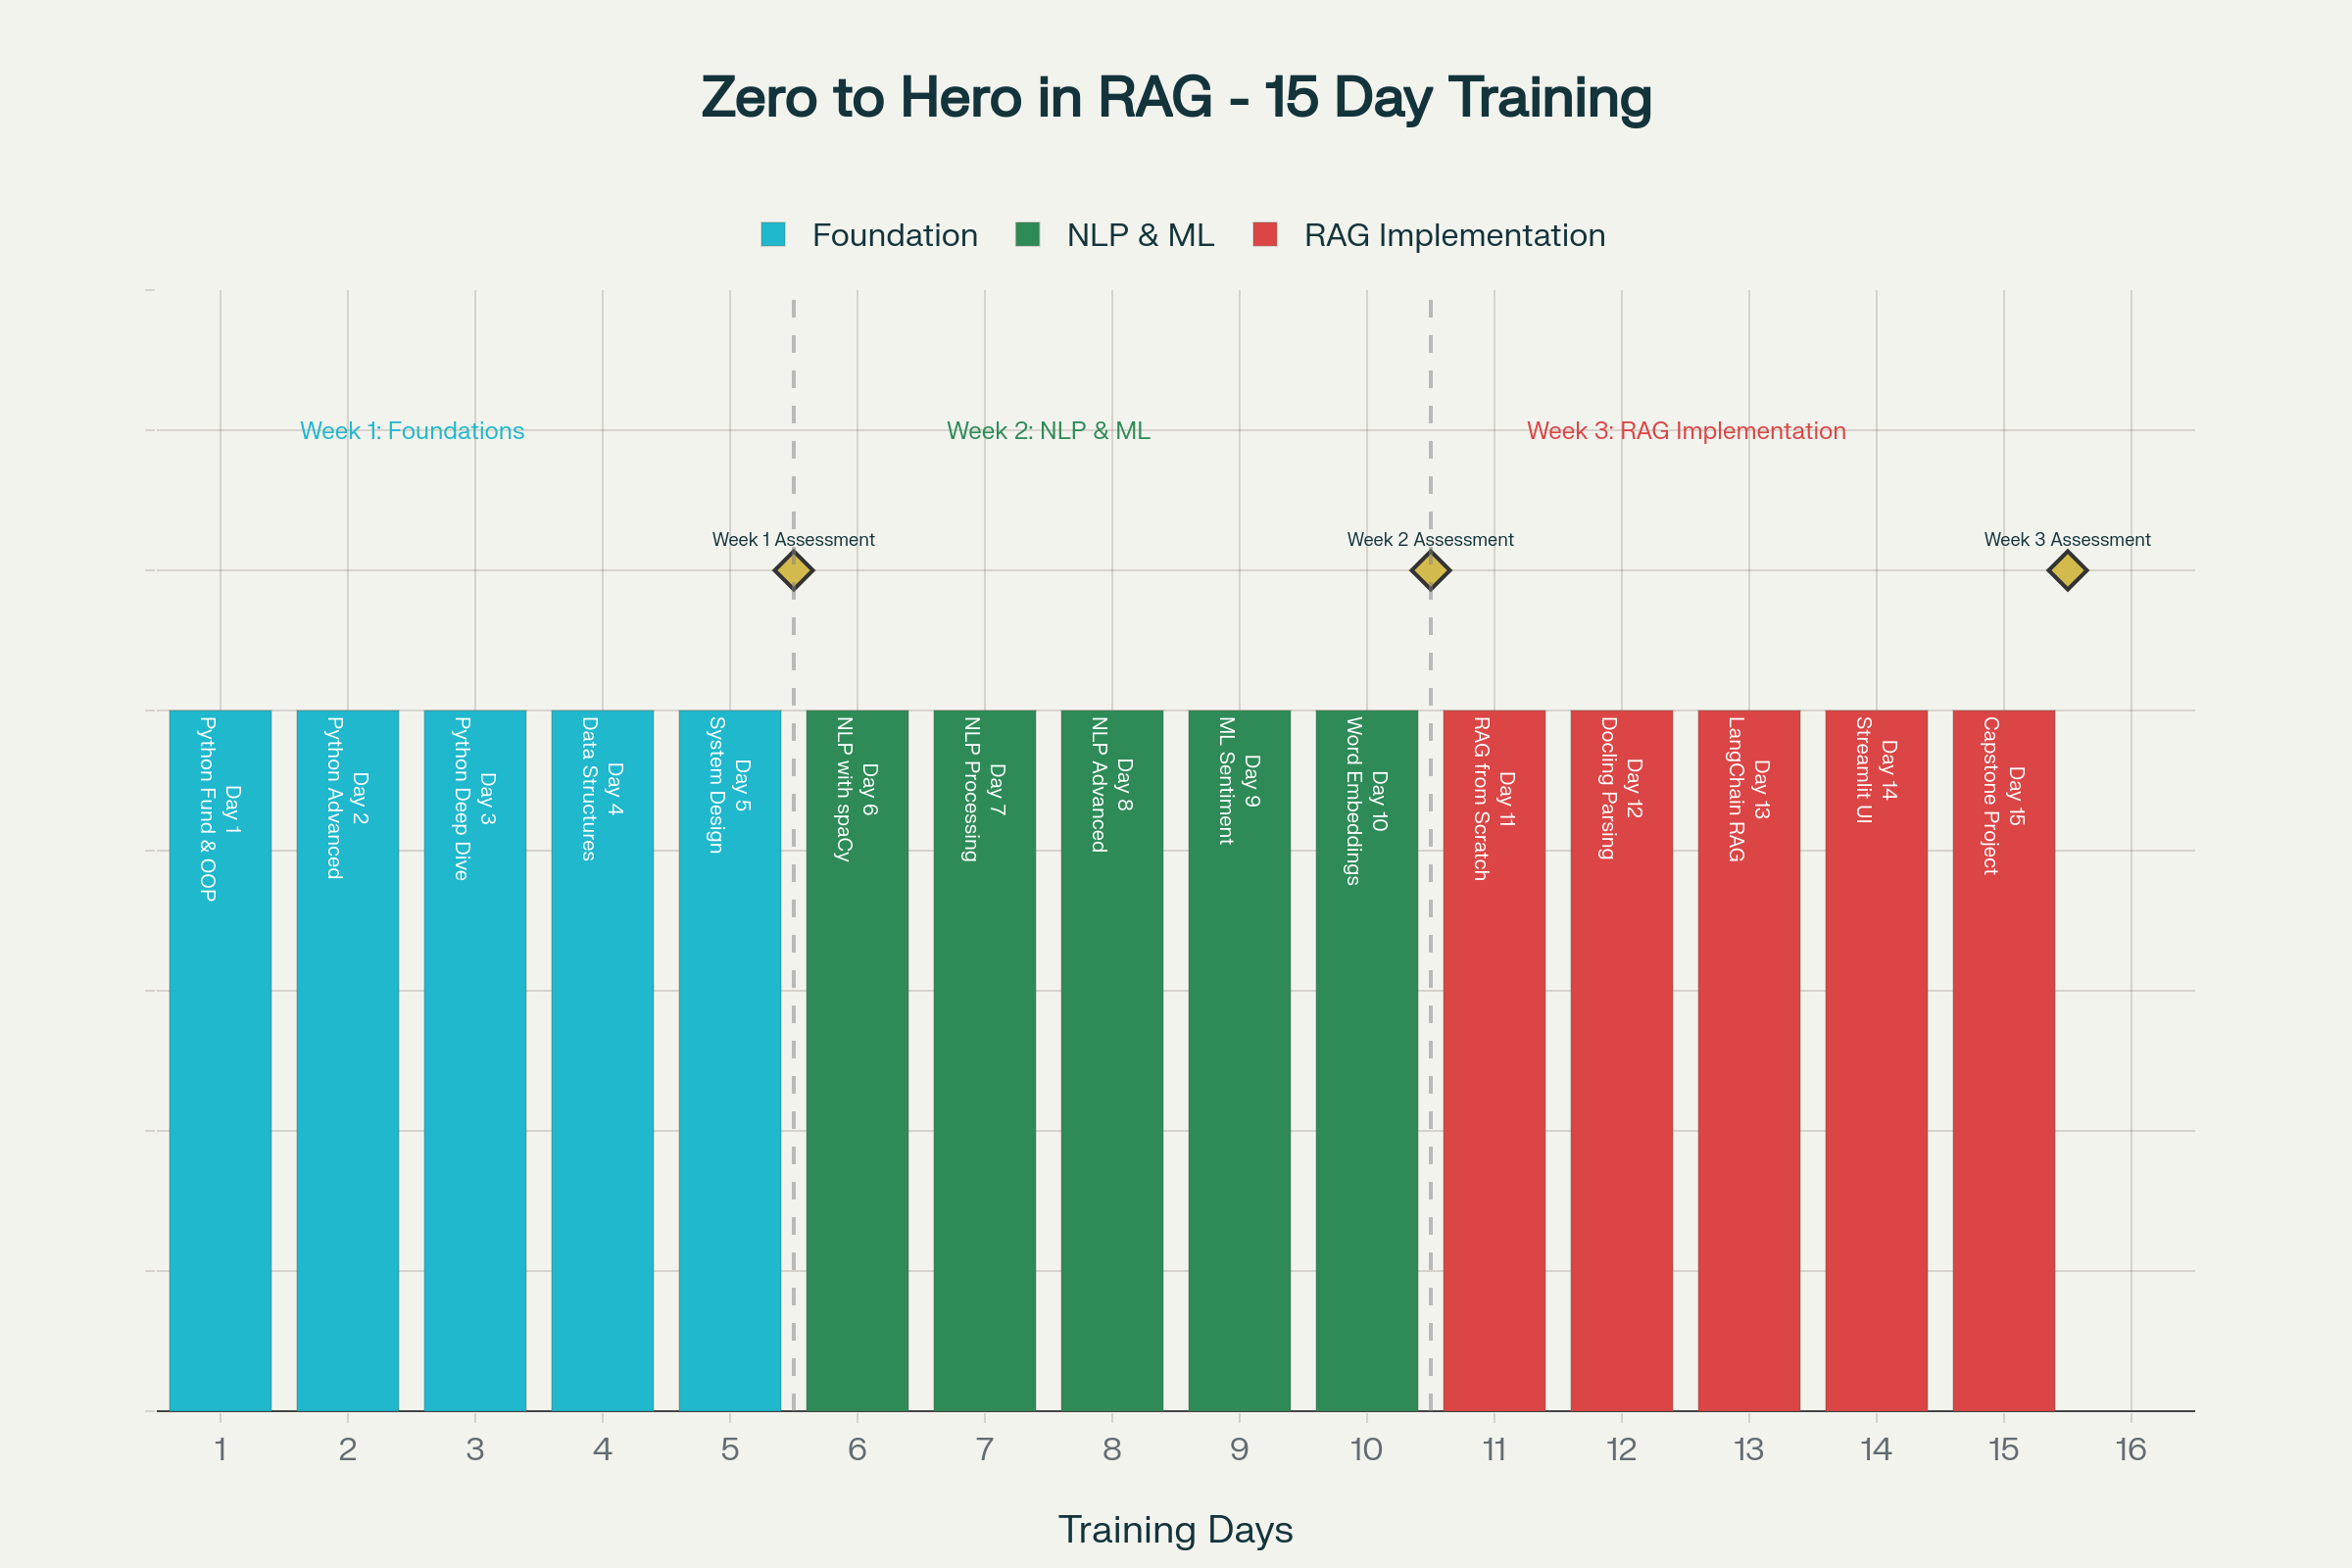
\includegraphics[width=\linewidth,keepaspectratio]{zero2hero_rag_1}
		\end{center}
\end{frame}

%%%%%%%%%%%%%%%%%%%%%%%%%%%%%%%%%%%%%%%%%%%%%%%%%%%%%%%%%%%%%%%%%%%%%
% SLIDE 1: TITLE SLIDE
%%%%%%%%%%%%%%%%%%%%%%%%%%%%%%%%%%%%%%%%%%%%%%%%%%%%%%%%%%%%%%%%%%%%%
\begin{frame}[fragile]\frametitle{From Zero to Hero in RAG}

\textbf{Learning Path:} Python $\rightarrow$ DSA $\rightarrow$ System Design $\rightarrow$ NLP $\rightarrow$ RAG $\rightarrow$ Prod
\vspace{0.3cm}  


\begin{columns}
    \begin{column}[T]{0.6\linewidth}
      \textbf{Program Overview}
      \begin{itemize}
        \item Duration: 15 working days (3 weeks)
        \item Daily: 8 hours (4 learning + 4 coding)
        \item Target: Software engineers with basic programming knowledge
      \end{itemize}
    \end{column}
    \begin{column}[T]{0.4\linewidth}
      \textbf{What You'll Build}
      \begin{itemize}
        \item 15 progressive projects
        \item 1 production capstone
        \item Complete end-to-end RAG
      \end{itemize}
    \end{column}
  \end{columns}
  


\vspace{0.3cm}  
\textbf{Portfolio Highlights:}
      \begin{itemize}
        \item Week 1: 5 Python projects + System design
        \item Week 2: NLP pipeline + ML model + Embeddings
        \item Week 3: Production RAG system with UI
      \end{itemize}		
\end{frame}

%%%%%%%%%%%%%%%%%%%%%%%%%%%%%%%%%%%%%%%%%%%%%%%%%%%%%%%%%%%%%%%%%%%%%
% SLIDE 2: PROGRAM STRUCTURE
%%%%%%%%%%%%%%%%%%%%%%%%%%%%%%%%%%%%%%%%%%%%%%%%%%%%%%%%%%%%%%%%%%%%%
\begin{frame}[fragile]\frametitle{Program Architecture}
\begin{columns}
    \begin{column}[T]{0.33\linewidth}
      \textbf{Phase 1: Foundations}
      \textbf{(Days 1-5)}
      \begin{itemize}
        \item Python Fundas
        \item Advanced Python
        \item DSA Algorithms
        \item System Design
      \end{itemize}
    \end{column}
    \begin{column}[T]{0.33\linewidth}
      \textbf{Phase 2: NLP \& ML}
      \textbf{(Days 6-10)}
      \begin{itemize}
        \item spaCy NLP
        \item Text Processing
        \item Sentiment Analysis
        \item Word Embeddings
      \end{itemize}
    \end{column}
    \begin{column}[T]{0.33\linewidth}
      \textbf{Phase 3: RAG}
      \textbf{(Days 11-15)}
      \begin{itemize}
        \item RAG from Scratch
        \item Docling Parsing
        \item LangChain RAG
        \item Streamlit UI
      \end{itemize}
    \end{column}
  \end{columns}
  
\vspace{0.3cm}    
\textbf{Daily Structure:}
\begin{itemize}
  \item 09:00-13:00: Learning (concept + guided examples)
  \item 14:00-18:00: Coding (project implementation)
  \item Thursday 16:00-17:00: Weekly QnA Session
\end{itemize}  
\end{frame}

%%%%%%%%%%%%%%%%%%%%%%%%%%%%%%%%%%%%%%%%%%%%%%%%%%%%%%%%%%%%%%%%%%%%%
% SLIDE 3: DAY 1 - PYTHON OOP
%%%%%%%%%%%%%%%%%%%%%%%%%%%%%%%%%%%%%%%%%%%%%%%%%%%%%%%%%%%%%%%%%%%%%
\begin{frame}[fragile]\frametitle{Day 1: Python Fundamentals \& OOP}
\begin{columns}
    \begin{column}[T]{0.5\linewidth}
      \textbf{Morning Session (4 hrs)}
      \begin{itemize}
        \item Variables \& data types
        \item Control flow (if, loops)
        \item Functions \& scope
        \item Object-oriented programming
        \item Inheritance \& polymorphism
      \end{itemize}
    \end{column}
    \begin{column}[T]{0.5\linewidth}
      \textbf{Afternoon: Pick 1 Project}
      \begin{itemize}
        \item Shopping Cart System
        \item Employment Hierarchy
        \item Library Management
        \item Game tic-tac-toe
        \item Banking System
      \end{itemize}
    \end{column}
  \end{columns}
  
  \vspace{0.3cm}
  \textbf{Resources (Free):}
  \begin{itemize}
    \item Google's Python Class (https://developers.google.com/edu/python)
    \item Python Essentials (https://pythoninstitute.org/)
    \item Real Python OOP (realpython.com)
  \end{itemize}
  
\vspace{0.3cm}  
\textbf{Difficulty:} Medium \textbar \textbf{Time:} 4 hours \textbar \textbf{Deliverable:} Working code  
\end{frame}

%%%%%%%%%%%%%%%%%%%%%%%%%%%%%%%%%%%%%%%%%%%%%%%%%%%%%%%%%%%%%%%%%%%%%
% SLIDE 4: DAY 2 - ADVANCED PYTHON
%%%%%%%%%%%%%%%%%%%%%%%%%%%%%%%%%%%%%%%%%%%%%%%%%%%%%%%%%%%%%%%%%%%%%
\begin{frame}[fragile]\frametitle{Day 2: Advanced Python \& File Handling}
\begin{columns}
    \begin{column}[T]{0.5\linewidth}
      \textbf{Morning Session (4 hrs)}
      \begin{itemize}
        \item Decorators
        \item Generators \& iterators
        \item Context managers
        \item Exception handling
        \item File I/O, JSON, CSV
      \end{itemize}
    \end{column}
    \begin{column}[T]{0.5\linewidth}
      \textbf{Afternoon: Pick 1 Project}
      \begin{itemize}
        \item Logging decorators
        \item CSV data processor
        \item File backup system
        \item Config file manager
        \item Validation decorators
      \end{itemize}
    \end{column}
  \end{columns}
  
  \vspace{0.3cm}
  \textbf{Resources (Free):}
  \begin{itemize}
    \item Real Python Decorators (realpython.com/decorators)
    \item W3Schools File Handling (w3schools.com/python/file)
    \item DataCamp Data Processing (freemium)
  \end{itemize}
  
\vspace{0.3cm}    
\textbf{Difficulty:} Medium \textbar \textbf{Time:} 4 hours \textbar \textbf{Deliverable:} Working code  
\end{frame}

%%%%%%%%%%%%%%%%%%%%%%%%%%%%%%%%%%%%%%%%%%%%%%%%%%%%%%%%%%%%%%%%%%%%%
% SLIDE 5: DAY 3 - ADVANCED DEEP DIVE
%%%%%%%%%%%%%%%%%%%%%%%%%%%%%%%%%%%%%%%%%%%%%%%%%%%%%%%%%%%%%%%%%%%%%
\begin{frame}[fragile]\frametitle{Day 3: Python Advanced Deep Dive}
\begin{columns}
    \begin{column}[T]{0.5\linewidth}
      \textbf{Morning Session (4 hrs)}
      \begin{itemize}
        \item Metaclasses
        \item Descriptors
        \item Comprehensions
        \item Async/await
        \item Memory management
        \item Performance optimization
      \end{itemize}
    \end{column}
    \begin{column}[T]{0.5\linewidth}
      \textbf{Afternoon: Pick 1 Project}
      \begin{itemize}
        \item Async web scraper
        \item Lazy-loading properties
        \item Concurrent file processor
        \item Generator ETL pipeline
        \item Thread-safe cache
      \end{itemize}
    \end{column}
  \end{columns}
  
  \vspace{0.3cm}
  \textbf{Resources (Free):}
  \begin{itemize}
    \item Real Python Concurrency (realpython.com/concurrency)
    \item Fluent Python concepts (github.com/fluentpython)
    \item Memory Management (realpython.com/memory)
  \end{itemize}

\vspace{0.3cm}    
\textbf{Difficulty:} Medium \textbar \textbf{Time:} 4 hours \textbar \textbf{Deliverable:} Working code  
\end{frame}

%%%%%%%%%%%%%%%%%%%%%%%%%%%%%%%%%%%%%%%%%%%%%%%%%%%%%%%%%%%%%%%%%%%%%
% SLIDE 6: DAY 4 - DSA & ALGORITHMS
%%%%%%%%%%%%%%%%%%%%%%%%%%%%%%%%%%%%%%%%%%%%%%%%%%%%%%%%%%%%%%%%%%%%%
\begin{frame}[fragile]\frametitle{Day 4: Data Structures \& Algorithms}
\begin{columns}
    \begin{column}[T]{0.5\linewidth}
      \textbf{Morning Session (4 hrs)}
      \begin{itemize}
        \item Arrays, linked lists
        \item Stacks, queues
        \item Sorting algorithms
        \item Searching algorithms
        \item Big O complexity
        \item Time/space analysis
      \end{itemize}
    \end{column}
    \begin{column}[T]{0.5\linewidth}
      \textbf{Afternoon: Pick 1 Project}
      \begin{itemize}
        \item Linked list (LeetCode 206)
        \item 5 LeetCode problems
        \item Sorting algorithms
        \item Expression evaluation
        \item Hash map problems
      \end{itemize}
    \end{column}
  \end{columns}
  
  \vspace{0.3cm}
  \textbf{Resources (Free):}
  \begin{itemize}
    \item W3Schools DSA (w3schools.com/dsa)
    \item GeeksforGeeks (geeksforgeeks.org/dsa)
    \item LeetCode Explore (leetcode.com/explore)
  \end{itemize}

\vspace{0.3cm}    
\textbf{Difficulty:} Medium \textbar \textbf{Time:} 4 hours \textbar \textbf{Deliverable:} Working code  
\end{frame}

%%%%%%%%%%%%%%%%%%%%%%%%%%%%%%%%%%%%%%%%%%%%%%%%%%%%%%%%%%%%%%%%%%%%%
% SLIDE 7: DAY 5 - SYSTEM DESIGN
%%%%%%%%%%%%%%%%%%%%%%%%%%%%%%%%%%%%%%%%%%%%%%%%%%%%%%%%%%%%%%%%%%%%%
\begin{frame}[fragile]\frametitle{Day 5: System Design Fundamentals}
\begin{columns}
    \begin{column}[T]{0.5\linewidth}
      \textbf{Morning Session (4 hrs)}
      \begin{itemize}
        \item Requirements clarification
        \item Scalability patterns
        \item Caching strategies
        \item Load balancing
        \item Database design
        \item CAP theorem
      \end{itemize}
    \end{column}
    \begin{column}[T]{0.5\linewidth}
      \textbf{Afternoon: Pick 1 Project}
      \begin{itemize}
        \item URL shortener (TinyURL)
        \item Real-time chat system
        \item API rate limiter
        \item Real-time leaderboard
        \item Notification system
      \end{itemize}
    \end{column}
  \end{columns}
  
  \vspace{0.3cm}
  \textbf{Resources (Free):}
  \begin{itemize}
    \item System Design Handbook (algomaster.io)
    \item DesignGurus Guide (designgurus.io)
    \item InterviewBit (interviewbit.com)
  \end{itemize}
  
\vspace{0.3cm}    
\textbf{Difficulty:} Medium \textbar \textbf{Time:} 4 hours \textbar \textbf{Deliverable:} Working code  
\end{frame}

%%%%%%%%%%%%%%%%%%%%%%%%%%%%%%%%%%%%%%%%%%%%%%%%%%%%%%%%%%%%%%%%%%%%%
% SLIDE 8: WEEK 1 MILESTONE
%%%%%%%%%%%%%%%%%%%%%%%%%%%%%%%%%%%%%%%%%%%%%%%%%%%%%%%%%%%%%%%%%%%%%
\begin{frame}[fragile]\frametitle{Week 1 Milestone Assessment}
\begin{columns}
    \begin{column}[T]{0.5\linewidth}
      \textbf{Learning Outcomes}
      \begin{itemize}
        \item Python OOP mastery
        \item Advanced patterns
        \item DSA competency
        \item System thinking
      \end{itemize}
    \end{column}
    \begin{column}[T]{0.5\linewidth}
      \textbf{Success Criteria}
      \begin{itemize}
        \item 5 projects completed
        \item Core concepts understood
        \item Code quality >80\%
        \item Ready for NLP phase
      \end{itemize}
    \end{column}
  \end{columns}
  
  \vspace{0.3cm}
  \textbf{Assessment Activities:}
  \begin{itemize}
    \item Code review of all 5 projects
    \item Technical Q\&A on concepts
    \item System design explanation
    \item Readiness verification
  \end{itemize}
  
\vspace{0.3cm}
\textbf{Assessment Rubric:}
\begin{itemize}
  \item Functionality (50 pts) - All features working
  \item Code Quality (20 pts) - Clean, documented
  \item Design Principles (20 pts) - Architecture
  \item Presentation (10 pts) - Documentation quality
\end{itemize}  
\end{frame}

%%%%%%%%%%%%%%%%%%%%%%%%%%%%%%%%%%%%%%%%%%%%%%%%%%%%%%%%%%%%%%%%%%%%%
% SLIDE 9: DAY 6 - NLP WITH SPACY
%%%%%%%%%%%%%%%%%%%%%%%%%%%%%%%%%%%%%%%%%%%%%%%%%%%%%%%%%%%%%%%%%%%%%
\begin{frame}[fragile]\frametitle{Day 6: NLP Basics with spaCy}
\begin{columns}
    \begin{column}[T]{0.5\linewidth}
      \textbf{Morning Session (4 hrs)}
      \begin{itemize}
        \item NLP fundamentals
        \item spaCy pipeline
        \item Tokenization
        \item POS tagging
        \item Named Entity Recognition
      \end{itemize}
    \end{column}
    \begin{column}[T]{0.5\linewidth}
      \textbf{Afternoon: Pick 1 Project}
      \begin{itemize}
        \item Text tokenizer
        \item NER system
        \item Text similarity
        \item Dependency parser
        \item Entity linker
      \end{itemize}
    \end{column}
  \end{columns}
  
  \vspace{0.3cm}
  \textbf{Resources (Free):}
  \begin{itemize}
    \item spaCy Advanced Course (course.spacy.io)
    \item Real Python spaCy (realpython.com/spacy)
    \item GeeksforGeeks NLP (geeksforgeeks.org/nlp)
  \end{itemize}
\end{frame}

%%%%%%%%%%%%%%%%%%%%%%%%%%%%%%%%%%%%%%%%%%%%%%%%%%%%%%%%%%%%%%%%%%%%%
% SLIDE 10: DAY 7 - NLP PROCESSING
%%%%%%%%%%%%%%%%%%%%%%%%%%%%%%%%%%%%%%%%%%%%%%%%%%%%%%%%%%%%%%%%%%%%%
\begin{frame}[fragile]\frametitle{Day 7: NLP Processing \& Text Analysis}
\begin{columns}
    \begin{column}[T]{0.5\linewidth}
      \textbf{Morning Session (4 hrs)}
      \begin{itemize}
        \item Text preprocessing
        \item Lemmatization
        \item Stop word removal
        \item Text normalization
        \item TF-IDF vectorization
        \item Feature extraction
      \end{itemize}
    \end{column}
    \begin{column}[T]{0.5\linewidth}
      \textbf{Afternoon: Pick 1 Project}
      \begin{itemize}
        \item Preprocessing pipeline
        \item TF-IDF vectorizer
        \item Advanced text cleaner
        \item Keyword extractor
        \item Document summarizer
      \end{itemize}
    \end{column}
  \end{columns}
  
  \vspace{0.3cm}
  \textbf{Resources (Free):}
  \begin{itemize}
    \item Real Python Text Processing (realpython.com)
    \item NLTK Documentation (nltk.org)
    \item DataCamp Text Analytics (freemium)
  \end{itemize}
\end{frame}

%%%%%%%%%%%%%%%%%%%%%%%%%%%%%%%%%%%%%%%%%%%%%%%%%%%%%%%%%%%%%%%%%%%%%
% SLIDE 11: DAY 8 - ADVANCED NLP
%%%%%%%%%%%%%%%%%%%%%%%%%%%%%%%%%%%%%%%%%%%%%%%%%%%%%%%%%%%%%%%%%%%%%
\begin{frame}[fragile]\frametitle{Day 8: NLP Advanced Topics}
\begin{columns}
    \begin{column}[T]{0.5\linewidth}
      \textbf{Morning Session (4 hrs)}
      \begin{itemize}
        \item Dependency parsing
        \item Syntax trees
        \item Coreference resolution
        \item Topic modeling
        \item Information extraction
        \item Semantic role labeling
      \end{itemize}
    \end{column}
    \begin{column}[T]{0.5\linewidth}
      \textbf{Afternoon: Pick 1 Project}
      \begin{itemize}
        \item Syntax parser
        \item Coreference resolution
        \item Relation extraction
        \item Semantic role labeler
        \item QA system (template-based)
      \end{itemize}
    \end{column}
  \end{columns}
  
  \vspace{0.3cm}
  \textbf{Resources (Free):}
  \begin{itemize}
    \item Advanced spaCy Course (course.spacy.io)
    \item Real Python NLP (realpython.com)
    \item GeeksforGeeks Advanced (geeksforgeeks.org/nlp)
  \end{itemize}
\end{frame}

%%%%%%%%%%%%%%%%%%%%%%%%%%%%%%%%%%%%%%%%%%%%%%%%%%%%%%%%%%%%%%%%%%%%%
% SLIDE 12: DAY 9 - ML SENTIMENT ANALYSIS
%%%%%%%%%%%%%%%%%%%%%%%%%%%%%%%%%%%%%%%%%%%%%%%%%%%%%%%%%%%%%%%%%%%%%
\begin{frame}[fragile]\frametitle{Day 9: Machine Learning + Sentiment Analysis}
\begin{columns}
    \begin{column}[T]{0.5\linewidth}
      \textbf{Morning Session (4 hrs)}
      \begin{itemize}
        \item Sentiment analysis approaches
        \item Feature engineering
        \item ML classifiers
        \item Model evaluation
        \item Imbalanced datasets
        \item Ensemble methods
      \end{itemize}
    \end{column}
    \begin{column}[T]{0.5\linewidth}
      \textbf{Afternoon: Pick 1 Project}
      \begin{itemize}
        \item Lexicon-based analyzer
        \item ML classifier
        \item Ensemble model
        \item Real-time analyzer
        \item Aspect-based sentiment
      \end{itemize}
    \end{column}
  \end{columns}
  
  \vspace{0.3cm}
  \textbf{Resources (Free):}
  \begin{itemize}
    \item DataCamp NLTK (datacamp.com/tutorial/nltk)
    \item Real Python Sentiment (realpython.com/sentiment)
    \item Towards Data Science (towardsdatascience.com)
  \end{itemize}
\end{frame}

%%%%%%%%%%%%%%%%%%%%%%%%%%%%%%%%%%%%%%%%%%%%%%%%%%%%%%%%%%%%%%%%%%%%%
% SLIDE 13: DAY 10 - WORD EMBEDDINGS
%%%%%%%%%%%%%%%%%%%%%%%%%%%%%%%%%%%%%%%%%%%%%%%%%%%%%%%%%%%%%%%%%%%%%
\begin{frame}[fragile]\frametitle{Day 10: Word Embeddings}
\begin{columns}
    \begin{column}[T]{0.5\linewidth}
      \textbf{Morning Session (4 hrs)}
      \begin{itemize}
        \item Word2Vec (CBOW, Skip-Gram)
        \item GloVe embeddings
        \item FastText
        \item Embedding visualization
        \item Pre-trained models
        \item Transfer learning
      \end{itemize}
    \end{column}
    \begin{column}[T]{0.5\linewidth}
      \textbf{Afternoon: Pick 1 Project}
      \begin{itemize}
        \item Word2Vec training
        \item Analogy solver
        \item Document similarity
        \item t-SNE visualization
        \item Semantic search engine
      \end{itemize}
    \end{column}
  \end{columns}
  
  \vspace{0.3cm}
  \textbf{Resources (Free):}
  \begin{itemize}
    \item GeeksforGeeks Word2Vec (geeksforgeeks.org)
    \item Milvus Embeddings (milvus.io)
    \item TensorFlow Word2Vec (tensorflow.org)
  \end{itemize}
\end{frame}

%%%%%%%%%%%%%%%%%%%%%%%%%%%%%%%%%%%%%%%%%%%%%%%%%%%%%%%%%%%%%%%%%%%%%
% SLIDE 14: WEEK 2 MILESTONE
%%%%%%%%%%%%%%%%%%%%%%%%%%%%%%%%%%%%%%%%%%%%%%%%%%%%%%%%%%%%%%%%%%%%%
\begin{frame}[fragile]\frametitle{Week 2 Milestone Assessment}
\begin{columns}
    \begin{column}[T]{0.5\linewidth}
      \textbf{Learning Outcomes}
      \begin{itemize}
        \item NLP pipelines
        \item ML classification
        \item Embeddings mastery
        \item Semantic search
      \end{itemize}
    \end{column}
    \begin{column}[T]{0.5\linewidth}
      \textbf{Success Criteria}
      \begin{itemize}
        \item NLP pipeline functional
        \item ML model >80\% accuracy
        \item Embedding system works
        \item Ready for RAG phase
      \end{itemize}
    \end{column}
  \end{columns}
  
  \vspace{0.3cm}
  \textbf{Assessment Activities:}
  \begin{itemize}
    \item NLP pipeline demo
    \item Sentiment model evaluation
    \item Embedding visualization
    \item Component integration check
  \end{itemize}
\end{frame}

%%%%%%%%%%%%%%%%%%%%%%%%%%%%%%%%%%%%%%%%%%%%%%%%%%%%%%%%%%%%%%%%%%%%%
% SLIDE 15: DAY 11 - RAG FROM SCRATCH
%%%%%%%%%%%%%%%%%%%%%%%%%%%%%%%%%%%%%%%%%%%%%%%%%%%%%%%%%%%%%%%%%%%%%
\begin{frame}[fragile]\frametitle{Day 11: RAG from Scratch}
\begin{columns}
    \begin{column}[T]{0.5\linewidth}
      \textbf{Morning Session (4 hrs)}
      \begin{itemize}
        \item RAG architecture
        \item Vector stores
        \item Chunking strategies
        \item Retrieval mechanisms
        \item Re-ranking
        \item Integration patterns
      \end{itemize}
    \end{column}
    \begin{column}[T]{0.5\linewidth}
      \textbf{Afternoon: Pick 1 Project}
      \begin{itemize}
        \item Basic RAG system
        \item Document chunking
        \item Re-ranking retriever
        \item Full RAG pipeline
        \item Multi-doc RAG
      \end{itemize}
    \end{column}
  \end{columns}
  
  \vspace{0.3cm}
  \textbf{Resources (Free):}
  \begin{itemize}
    \item RAG from Scratch (linkedin.com/pulse)
    \item HuggingFace RAG (huggingface.co/blog)
    \item Glean RAG Guide (glean.com/blog)
  \end{itemize}
  
\textbf{Why RAG?} Combines retrieval with generation for:
\begin{itemize}
  \item Up-to-date information beyond training data
  \item Grounded, factual responses with citations
  \item Domain-specific knowledge integration
\end{itemize}
  
\textbf{Key Components:}
Document Loading → Chunking → Embedding → Vector Store → Retrieval → LLM → Response  
\end{frame}

%%%%%%%%%%%%%%%%%%%%%%%%%%%%%%%%%%%%%%%%%%%%%%%%%%%%%%%%%%%%%%%%%%%%%
% SLIDE 16: DAY 12 - DOCLING PARSING
%%%%%%%%%%%%%%%%%%%%%%%%%%%%%%%%%%%%%%%%%%%%%%%%%%%%%%%%%%%%%%%%%%%%%
\begin{frame}[fragile]\frametitle{Day 12: Docling Document Parsing}
\begin{columns}
    \begin{column}[T]{0.5\linewidth}
      \textbf{Morning Session (4 hrs)}
      \begin{itemize}
        \item Docling architecture
        \item PDF/DOCX/PPTX parsing
        \item Layout analysis
        \item OCR capabilities
        \item Table extraction
        \item Image extraction
      \end{itemize}
    \end{column}
    \begin{column}[T]{0.5\linewidth}
      \textbf{Afternoon: Pick 1 Project}
      \begin{itemize}
        \item Multi-format parser
        \item Table extractor
        \item Image extractor
        \item OCR processor
        \item Hierarchy extractor
      \end{itemize}
    \end{column}
  \end{columns}
  
  \vspace{0.3cm}
  \textbf{Resources (Free):}
  \begin{itemize}
    \item DataCamp Docling (datacamp.com/tutorial/docling)
    \item IBM Docling (github.com/docling-project)
    \item Geek Avenue (youtube.com - Docling Tutorial)
  \end{itemize}
\end{frame}

%%%%%%%%%%%%%%%%%%%%%%%%%%%%%%%%%%%%%%%%%%%%%%%%%%%%%%%%%%%%%%%%%%%%%
% SLIDE 17: DAY 13 - LANGCHAIN RAG
%%%%%%%%%%%%%%%%%%%%%%%%%%%%%%%%%%%%%%%%%%%%%%%%%%%%%%%%%%%%%%%%%%%%%
\begin{frame}[fragile]\frametitle{Day 13: LangChain RAG Implementation}
\begin{columns}
    \begin{column}[T]{0.5\linewidth}
      \textbf{Morning Session (4 hrs)}
      \begin{itemize}
        \item LangChain framework
        \item Document loaders
        \item Text splitters
        \item Embeddings integration
        \item Vector stores
        \item LCEL expressions
      \end{itemize}
    \end{column}
    \begin{column}[T]{0.5\linewidth}
      \textbf{Afternoon: Pick 1 Project}
      \begin{itemize}
        \item PDF Q\&A system
        \item Web scraping RAG
        \item Multi-index RAG
        \item Conversation RAG
        \item Advanced RAG
      \end{itemize}
    \end{column}
  \end{columns}
  
  \vspace{0.3cm}
  \textbf{Resources (Free):}
  \begin{itemize}
    \item LangChain RAG (python.langchain.com)
    \item Kody Simpson YouTube (youtube.com)
    \item DataCamp RAG (datacamp.com/courses)
  \end{itemize}
\end{frame}

%%%%%%%%%%%%%%%%%%%%%%%%%%%%%%%%%%%%%%%%%%%%%%%%%%%%%%%%%%%%%%%%%%%%%
% SLIDE 18: DAY 14 - STREAMLIT UI
%%%%%%%%%%%%%%%%%%%%%%%%%%%%%%%%%%%%%%%%%%%%%%%%%%%%%%%%%%%%%%%%%%%%%
\begin{frame}[fragile]\frametitle{Day 14: Streamlit UI Development}
\begin{columns}
    \begin{column}[T]{0.5\linewidth}
      \textbf{Morning Session (4 hrs)}
      \begin{itemize}
        \item Streamlit basics
        \item Layout components
        \item Interactive widgets
        \item Data visualization
        \item File uploads
        \item State management
      \end{itemize}
    \end{column}
    \begin{column}[T]{0.5\linewidth}
      \textbf{Afternoon: Pick 1 Project}
      \begin{itemize}
        \item Interactive dashboard
        \item Chatbot interface
        \item Document uploader
        \item RAG interface
        \item Multi-page app
      \end{itemize}
    \end{column}
  \end{columns}
  
  \vspace{0.3cm}
  \textbf{Resources (Free):}
  \begin{itemize}
    \item Streamlit Docs (docs.streamlit.io)
    \item GeeksforGeeks Streamlit (geeksforgeeks.org)
    \item DataQuest Chatbot (dataquest.io)
  \end{itemize}
\end{frame}

%%%%%%%%%%%%%%%%%%%%%%%%%%%%%%%%%%%%%%%%%%%%%%%%%%%%%%%%%%%%%%%%%%%%%
% SLIDE 19: DAY 15 - CAPSTONE PROJECT
%%%%%%%%%%%%%%%%%%%%%%%%%%%%%%%%%%%%%%%%%%%%%%%%%%%%%%%%%%%%%%%%%%%%%
\begin{frame}[fragile]\frametitle{Day 15: End-to-End Capstone Project}
\begin{columns}
    \begin{column}[T]{0.5\linewidth}
      \textbf{Morning Session (4 hrs)}
      \begin{itemize}
        \item Architecture planning
        \item Component integration
        \item Testing strategies
        \item Performance optimization
        \item Error handling
        \item Deployment prep
      \end{itemize}
    \end{column}
    \begin{column}[T]{0.5\linewidth}
      \textbf{Pick 1 Project (Full Stack)}
      \begin{itemize}
        \item Document Intelligence
        \item Advanced Multi-Doc RAG
        \item Enterprise Knowledge Base
        \item Real-Time Chat Analyzer
        \item AI Research Tool
      \end{itemize}
    \end{column}
  \end{columns}
  
\textbf{Integration Requirements:}
\begin{itemize}
  \item Docling: Multi-format document parsing
  \item LangChain: RAG orchestration \& chains
  \item Streamlit: Interactive web interface
  \item All components working together
\end{itemize}

\textbf{Capstone Evaluation (100 pts):}
Functionality (40) \textbar Code Quality (30) \textbar Architecture (20) \textbar Documentation (10)
\textbf{Minimum Score:} 70/100 to pass
\end{frame}

%%%%%%%%%%%%%%%%%%%%%%%%%%%%%%%%%%%%%%%%%%%%%%%%%%%%%%%%%%%%%%%%%%%%%
% SLIDE 20: WEEK 3 MILESTONE
%%%%%%%%%%%%%%%%%%%%%%%%%%%%%%%%%%%%%%%%%%%%%%%%%%%%%%%%%%%%%%%%%%%%%
\begin{frame}[fragile]\frametitle{Week 3 Milestone \& Final Assessment}
\begin{columns}
    \begin{column}[T]{0.5\linewidth}
      \textbf{Learning Outcomes}
      \begin{itemize}
        \item Complete RAG systems
        \item Document processing
        \item LLM orchestration
        \item Production applications
      \end{itemize}
    \end{column}
    \begin{column}[T]{0.5\linewidth}
      \textbf{Success Criteria}
      \begin{itemize}
        \item Capstone fully functional
        \item Code well-documented
        \item Architecture sound
        \item Production-ready
      \end{itemize}
    \end{column}
  \end{columns}
  
\textbf{Production Readiness Checklist:}
\begin{itemize}
  \item Error handling implemented
  \item Performance optimized
  \item Documentation complete
  \item Deployment configuration ready
\end{itemize}
  
  \vspace{0.3cm}
  \textbf{Final Assessment:}
  \begin{itemize}
    \item Capstone project demonstration
    \item Architecture explanation
    \item Code walkthrough
    \item Future enhancements discussion
  \end{itemize}
\end{frame}

%%%%%%%%%%%%%%%%%%%%%%%%%%%%%%%%%%%%%%%%%%%%%%%%%%%%%%%%%%%%%%%%%%%%%
% SLIDE 21: CLOSURE & NEXT STEPS
%%%%%%%%%%%%%%%%%%%%%%%%%%%%%%%%%%%%%%%%%%%%%%%%%%%%%%%%%%%%%%%%%%%%%
\begin{frame}[fragile]\frametitle{Congratulations! Next Steps}
\begin{columns}
    \begin{column}[T]{0.5\linewidth}
      \textbf{Technical Skills}
      \begin{itemize}
        \item Advanced Python
        \item NLP \& ML systems
        \item RAG architecture
        \item Full-stack development
      \end{itemize}
    \end{column}
    \begin{column}[T]{0.5\linewidth}
      \textbf{Career Pathways}
      \begin{itemize}
        \item AI/ML Engineer
        \item RAG Specialist
        \item LLM Infrastructure
        \item Product Engineer (AI)
      \end{itemize}
    \end{column}
  \end{columns}
  
  \vspace{0.3cm}
  \textbf{Next Certifications:}
  \begin{itemize}
    \item Azure AI Fundamentals (AI-900)
    \item LangChain Academy Certification
  \end{itemize}
  
\textbf{Continuous Learning Resources:}
\begin{itemize}
  \item LangChain Academy (academy.langchain.com)
  \item DeepLearning.AI Courses (deeplearning.ai)
  \item Hugging Face Course (huggingface.co/course)
  \item GitHub: Explore open source RAG projects
\end{itemize}
  
  \vspace{0.3cm}
  \textbf{Keep Building, Keep Learning!}
\end{frame}

